\addbibresource{reference.bib}

\chapter{Úvod}\label{chap01} 
Tato diplomová práce se zabývá návrhem a implementací softwarového systému \textbf{Pixnet} - software pro distribuované řízení sítě částicových pixelových detektorů. Software byl navržen především pro řízení detektorů \textit{Timepix3}, ale díky modulární architektuře je možné po implementaci potřebných modulů ho použít na řízení libovolného detektoru.

\section{Motivace}
\todo

\section{Timepix3 detektor}
Hybridní částicový pixelový detektor Timepix3\cite{timepix3} je nástupcem detektoru Timepix\cite{timepix} a je vyvíjen v rámci Medipix\footnoteUrl{http://medipix.web.cern.ch/} kolaborace v CERN, mezi jejíž členy patří od roku 1999 i ÚTEF ČVUT v Praze.

\begin{figure}[h]
    \begin{center}
        \begin{subfigure}{7.0cm}
            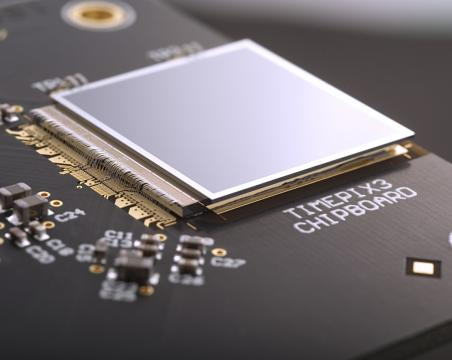
\includegraphics[width=7cm]{figures/timepix3.jpg}    
            \caption{Fotografie Timepix3 detektoru \cite{medipix_from_medical_img_to_space}.}
        \end{subfigure}
        \hspace{0.1cm}
        \begin{subfigure}{7.0cm}
            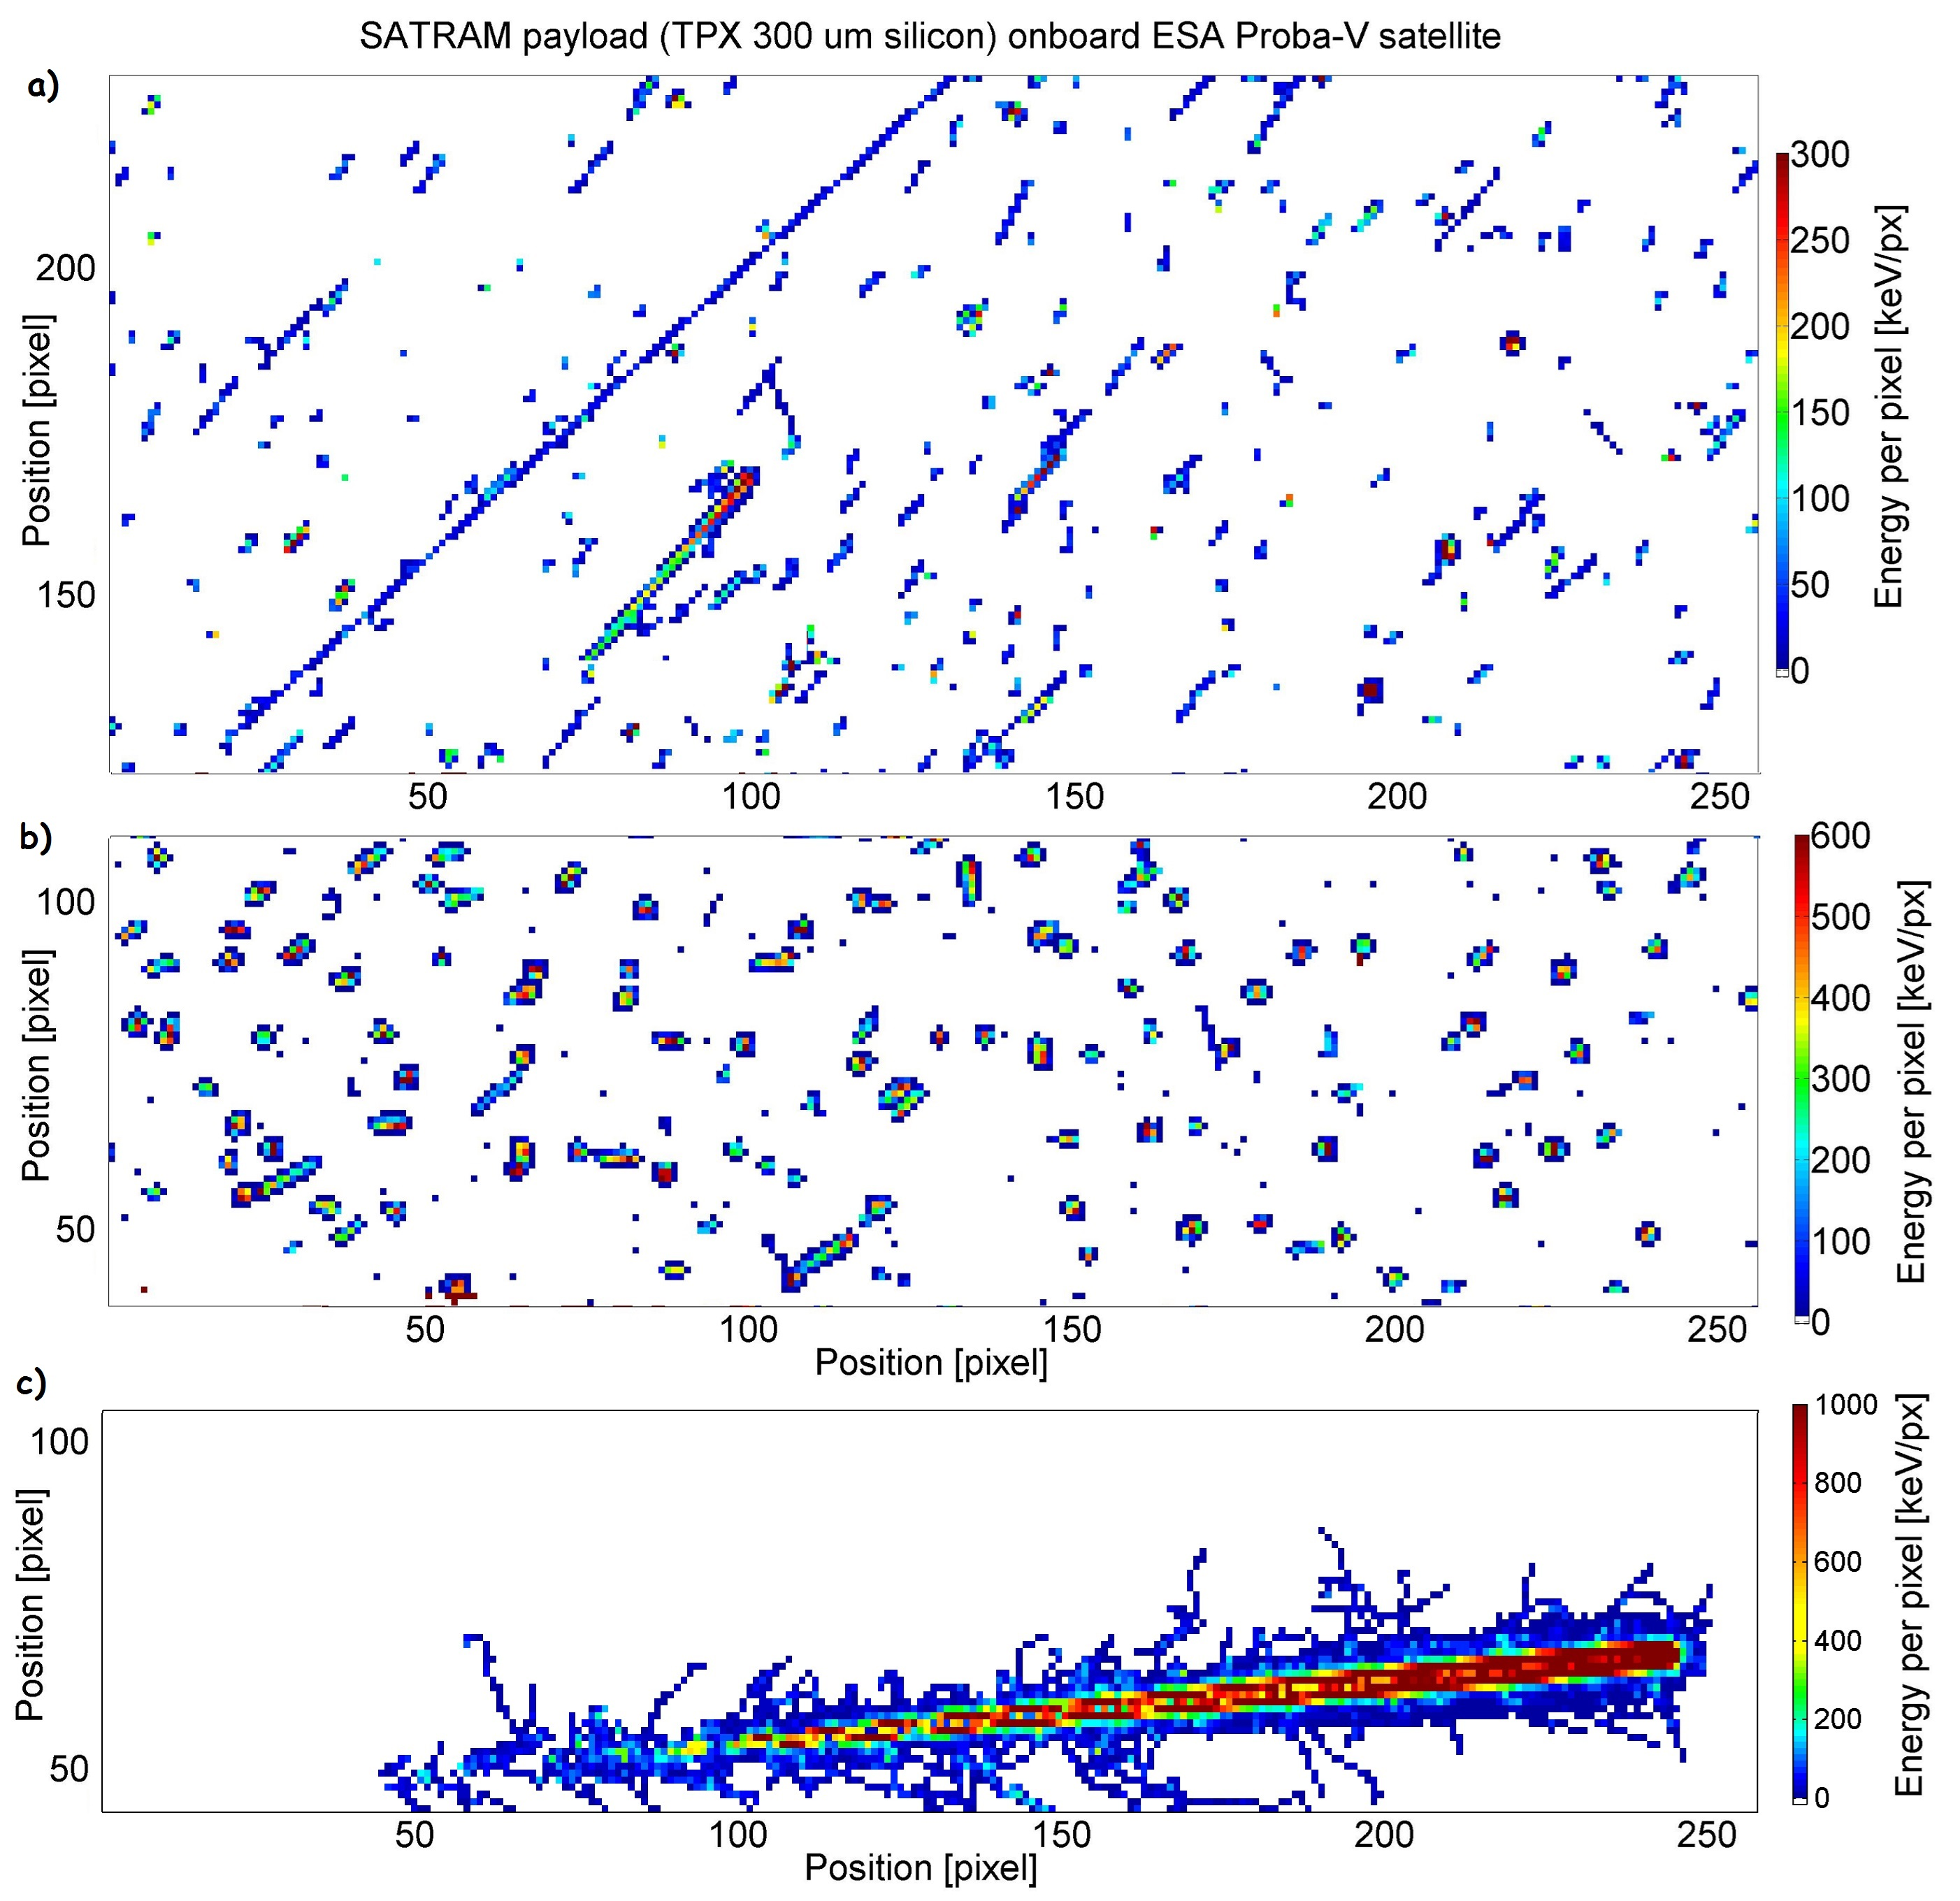
\includegraphics[width=7cm]{figures/timepix_data_satram.png}    
            \caption{Ukázka dat z detektoru Timepix, naměřených zařízením \textit{SATRAM}, které od roku 2013 obíhá Zemi na heliosynchronní kruhové polární dráze ve výšce \unit{820}{km} \cite{PlatkevicDisertace}.}
        \end{subfigure}
	\end{center}
    \caption{Detektor Timepix3 a vizualizace naměřeného vzorku dat.}
	\label{fig:master:frontend:detector_detail}
\end{figure}

Detektor se skládá z matice $256\times256$ nezávislých pixelů, každý o hraně $55~\mu m$. 
Jednotlivé pixely se skládají z citlivého polovodičového senzoru (nejčastěji \textit{Si}, nebo \textit{GaAs}) a vyčítací CMOS elektroniky (čítače, komparátory apod.). Princip funkce detektoru lze přirovnat digitálnímu fotoaparátu. Podobně jako u digitálního fotoaparátu, začátek a konec akvizice dat je řízen uzávěrkou (tzv. \textit{shutter signál}). Po tuto dobu pak citlivý polovodičový objem detektoru zaznamenává interakce s nabitými částicemi a dále je zpracovává dle nastaveného modu. V kapitole \ref{chap:detectors} bude na příklad popsán \textit{Time-Over-Threshold} mód, kde hodnota čítače pixelu na konci akvizice odpovídá deponované energii interagovaných částic s daným pixelem (mezi energií a TOT je nelineární závislost, která je dána fyzikálními vlastnostmi každého pixelu a je předmětem energetické kalibrace detektoru \cite{Jakubek2011S262}). 

Timepix3 detektor přináší oproti svému předchůdci několik výhod. Je schopný operovat i v kontinuálním módu, ve kterém je každý pixel detektoru schopný detekovanou událost ihned zpracovat, nezávisle na ostatních pixelech. Tím se téměř odstraňuje mrtvá doba detektoru, zvyšuje detekční účinnost, ale i zvyšuje datový tok z detektoru, jehož maximální teoretická hodnota je až $5.12 Gb/s$.

\section{Struktura práce}
\todo